

\documentclass[../../tc_tp3_main.tex]{subfiles}

\begin{document}

\hyphenation{di-fe-ren-cial}
\hyphenation{cons-tan-te}
\hyphenation{ins-tru-men-ta-ción}
\hyphenation{pro-pues-ta}
%capítulo, Amplificadores de instrumentación
\chapter{Amplificadores de instrumentación}

%Introducción
\section{Introducción}

	%Notación
	A modo de delimitar un marco teórico y notacional a partir del cual se presentarán con mayor claridad y precisión los términos técnicos siguientes, se procede a definir las dos entradas genéricas, $V_1$ y $V_2$, de un circuito de tipo MISO (multiple inputs, single output) como: \par
	
	%Notación V_{CM} + V_{DMi}
 	\begin{equation}
  	   \left\{
	  	    \begin{array}{ll}
		 					\mathrm{V_1} = \mathrm{V_{CM} + V_{DM1}} \\
			 				\mathrm{V_2} = \mathrm{V_{CM} + V_{DM2}} \\
	     	 \end{array}
	     	\right.
 	\end{equation}
 	
	donde $V_{CM}$ es la tensión de modo común, es decir, la componente compartida por las dos señales $V_1$ y $V_2$, y $V_{DMi}$ es la tensión diferencial o la componente única/diferente de la tensión i, con i =1;2.\par
	Nótese que tanto $V_{CM}$ como $V_{DMi}$ pueden ser nulas o no, dependiendo de las señales $V_1$ y $V_2$ y de la relación existente entre ellas. \par
	En particular, cuando la señal $V_1$ y $V_2$ comparten el mismo canal de transmisión se podrá decir que las señales comparten el ruido proveniente del canal y por lo tanto $V_{CM}$ será una variable aleatoria de distribución de probabilidad acorde, a determinar. Además, aquellas señales que estén montadas sobre tensiones continuas también tendrán una componente continua común. \par
	Debe también hacerse notar el hecho de que $V_1 - V_2 = V_{DM1} - V_{DM2}$, por lo que el modo común se verá eliminado al restar las dos señales de input. De aquí se desprende la notación a utilizar para el modo diferencial: $V_{DM} = V_{DM1} - V_{DM2}$\par
	Esta notación permite expresar a las entradas del sistema MISO como un circuito dispuesto de la siguiente forma:\par 
	%circuito VCM y VDM
	\begin{center}
	\begin{circuitikz}[american voltages]
	\draw
	(6,0) to [short, *-] (3,0)
  to [V, l_=$\frac{V_{DM}}{2}$] (3,3) 
  (6,6) to [short, *-] (3,6)
  to [V, l^= $\frac{V_{DM}}{2}$] (3,3) 
  to [V, l^= $V_{CM}$] (0,3) 
	(0,3) to (0,1) node[ground]{}; 
  \end{circuitikz}
  \end{center}
  
	Una vez establecida la notación anterior, procedemos a definir los siguientes términos:\par
	
	%definición de términos técnicos- itemize
	\begin{itemize}
	
	%definición amplificador diferencial
	\item Un \underline{amplificador diferencial} es un circuito cuya función será atenúar significativamente el modo común (idealmente eliminarlo) de las dos entradas y amplificar el modo diferencial de las mismas, realizando la diferencia entre las dos señales.\par
	En efecto, teniendo en cuenta la linealidad del sistema o circuito, se puede tratar al efecto sobre las entradas por superposición, por lo que definiendo a la ganancia del modo común a la salida del circuito como $A_{CM}$ y a la del modo diferencial como $A_{DM}$, si H es el efecto del sistema sobre las entradas, entonces $H(V_{1};V_{2}) = A_{DM} * V_{DM} + A_{CM} * V_{CM}$\par
	
	A continuación se presenta un modelo típico de un amplificador de diferencias. 
	
	%circuito amp diferencial
	\begin{figure}[H]	%ejemplo soft clipping
		\centering
		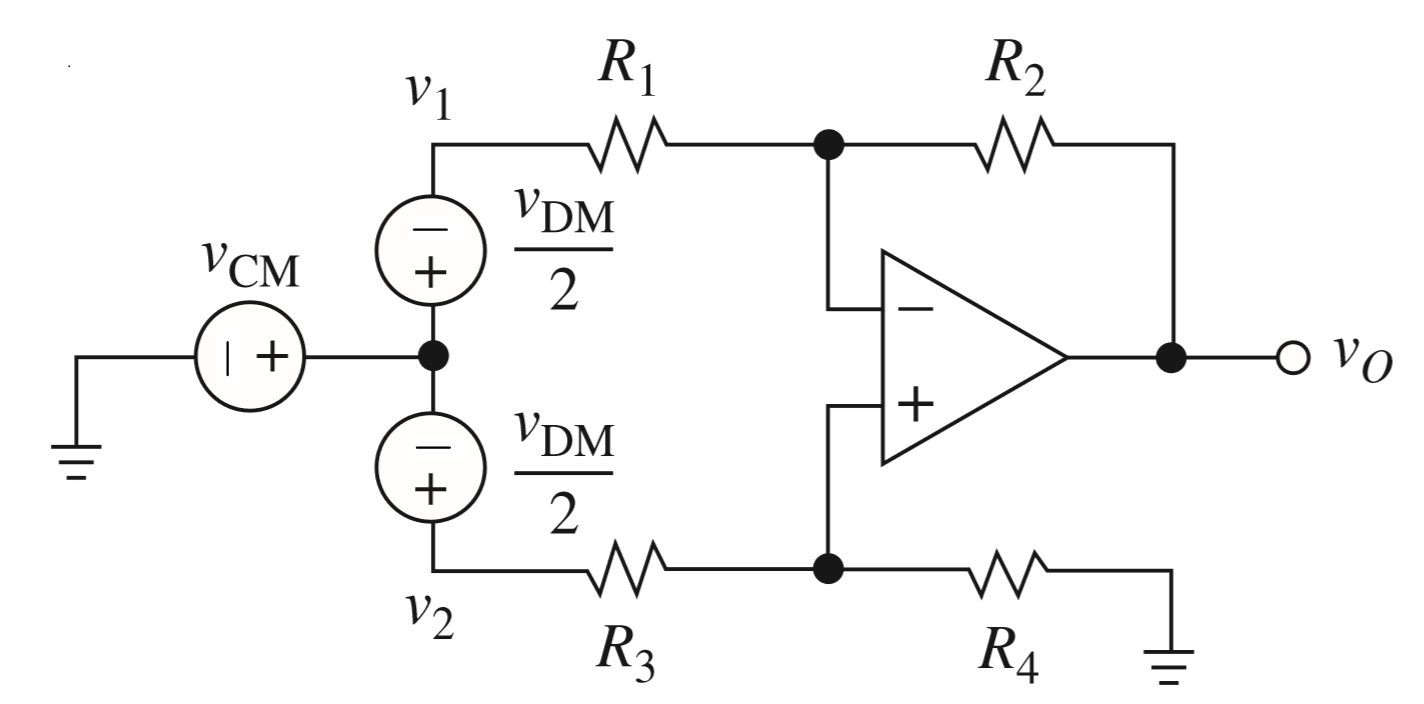
\includegraphics[scale=0.4]{imagenes/amp_diferencial.png}
		\caption{Modelo simple de amplificador diferencial}
		\label{fig:ej5_amp_diferencial}
	\end{figure}

	%definición CMRR
	\item El \underline{CMRR} o \underline{Common Mode Rejection Ratio} se define como la relación entre la ganancia del modo diferencial y el modo común, de forma tal que $CMRR =  \frac{A_{CM}}{A_{DM}}$. El mismo puede ser expresado en decibeles como $CMRR_{dB} =  20 \cdot \log_{10} {(\frac{A_{CM}}{A_{DM}})}$. \par
	La definición presentada anteriormente debe ser entendida entonces como una medida de cuánto prevalecerá el modo diferencial por sobre el modo común, es decir, permitirá cuantificar qué tan ''bueno'' es el amplificador diferencial: Cuanto mayor el CMRR, mejor cumple su función el  amplificador diferencial. Así, un amplificador diferencial ideal tendrá un CMRR infinito. \par
	
	%definición amplificador de instrumentación
	\item Un \underline{amplificador de instrumentación} es un amplificador diferencial que cumple con las siguientes condiciones: \par
	
	\begin{enumerate}
		\item Impedancia de entrada muy grande (idealmente infinita) tanto para el modo diferencial como para el común.
		\item Impedancia de salida muy baja (idealmente nula).
		\item Ganancia estable y precisa.
		\item Un CMRR extremadamente grande.
	\end{enumerate}
	Cabe destacar que si un amplificador de instrumentación utilizara el modelo de amplificador diferencial presentado anteriormente, las impedancia de entrada del circuito sería finita y en consecuencia se cargaría el resto del circuito. Esto resultaría en un deterioro  de las señales de entrada, perdiéndose la tensión ideal que estas proveerían. Es así como se degradaría el CMRR, ya que el modo común conformado por el ruido no sufriría pérdida mientras la señal diferencial sí lo haría.\par
	Para solucionar este problema, se inserta un buffer en cada entrada, con una impedancia de entrada resultante infinita idealmente que no deterioraría la señal de entrada.\par
	
	En este trabajo se justificará el uso del diseño de un amplificador instrumental propuesto por la cátedra, al cual se le asignará valores específicos para los componentes, justificando también la elección de dichos valores y analizando su comportamiento, intentando corroborar la relación de lo teórico y simulado con lo práctico.\par

%termino definiciones- itemize	
	\end{itemize}
	
%presento el circuito
\section{Diseño del amplificador de instrumentación}

La cátedra propone un circuito con el cual se implementará un amplificador de instrumentación. Los valores de los componentes serán determinados mediante un análisis completo y detallado del circuito. 

%Diseño del circuito propuesto
	\begin{figure}[H]	
		\centering
		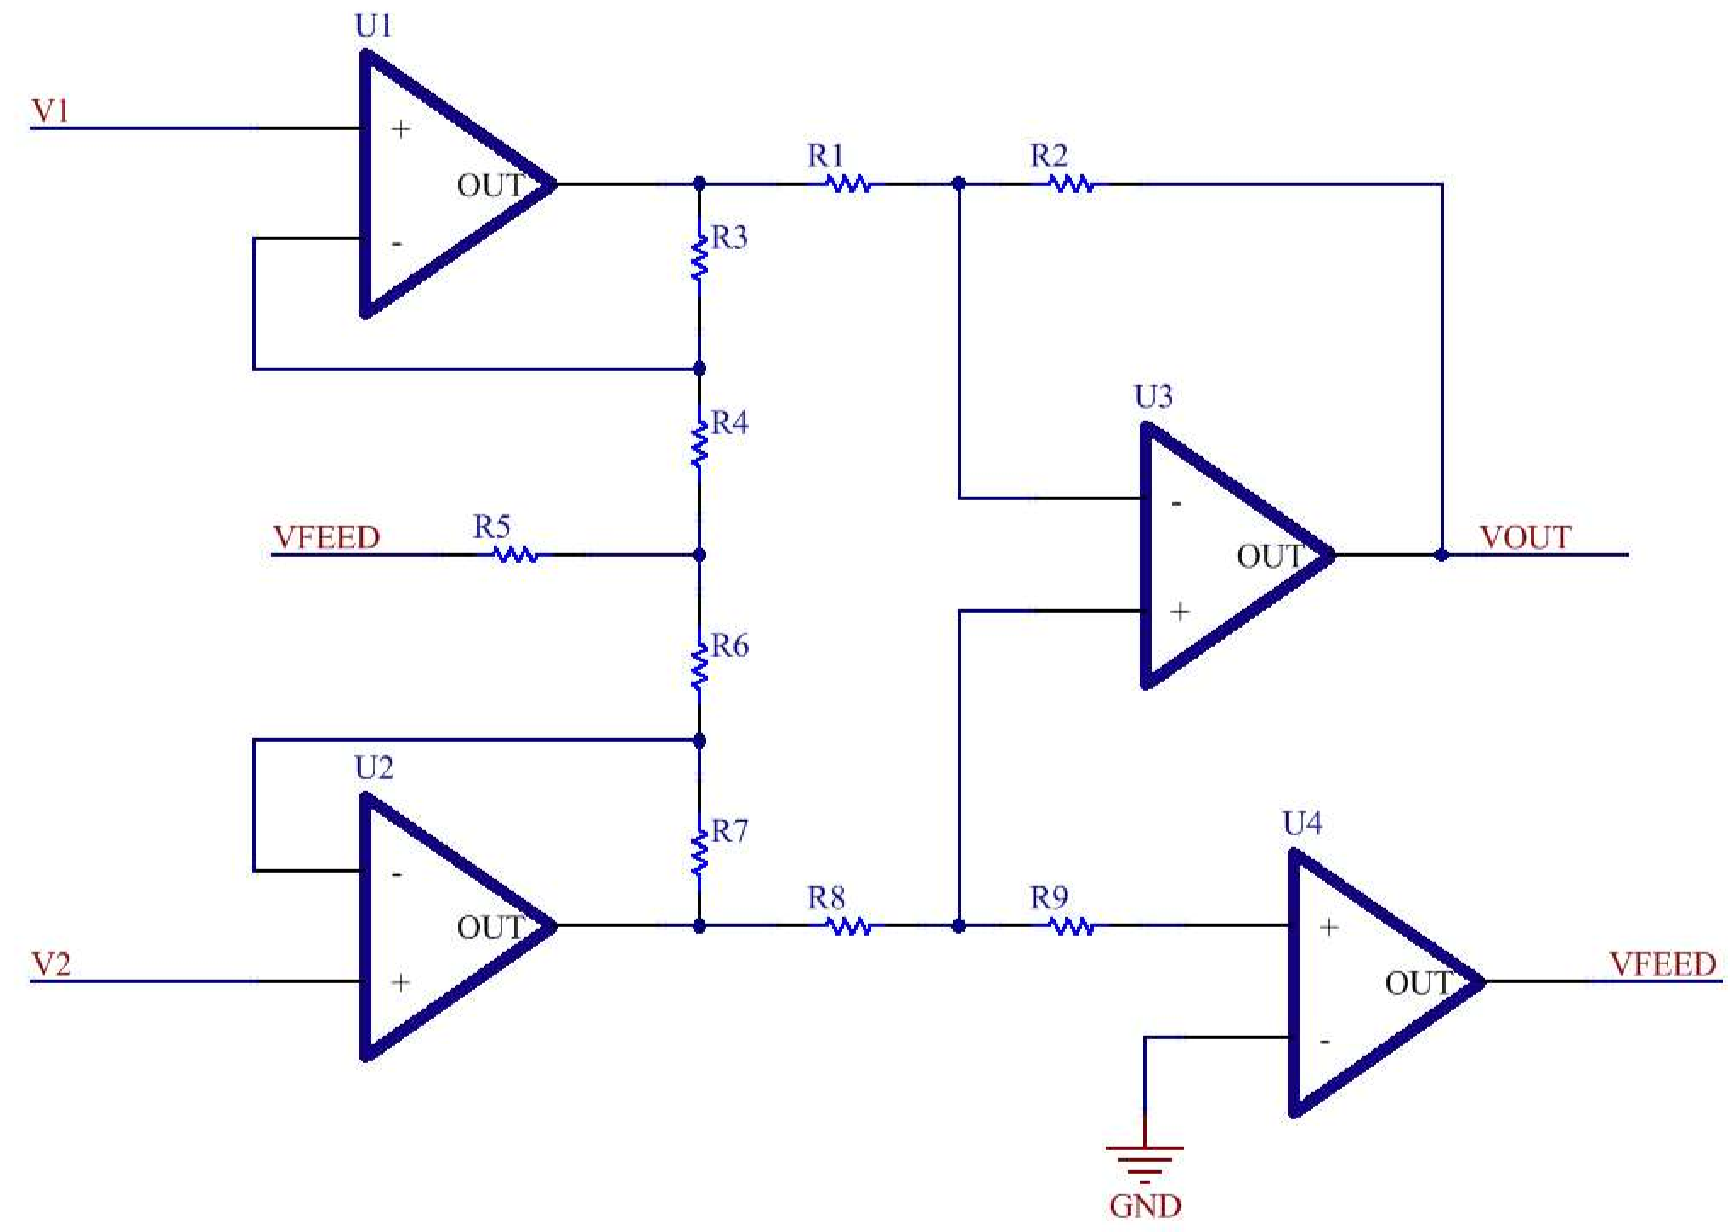
\includegraphics[scale=0.4]{imagenes/diseno_circuito.png}
		\caption{Circuito propuesto por la cátedra}
		\label{fig:ej3_diseno_circuito}
	\end{figure}
	
Al poseer 4 opamps, algunos con reatroalimentaciones entre sí, el tener en cuenta todas las no idealidades de estos 4 implicaría ecuaciones resultantes de alta complejidad y con tantas variables que el análisis sería engorroso y con pocas conclusiones que resulten de utilidad para los objetivos propuestos. Es por esto que las deducciones y los razonamientos con los cuales se podrá determinar los valores de los componentes para el buen funcionamiento del dispositivo provendrán de un análisis partido, con idealizaciones que se asuma contraerán un error bajo o aceptable y con algunos valores impuestos mediante la técnica de prueba y error a la hora de simular. \par
Primero, comenzaremos asumiendo que todos los opamps actúan bajo condiciones ideales.\par
	
%Análisis IDEAL del circuito
\subsection{Análisis ideal del circuito}

Para simplificar el análisis del circuito, como primer instancia se considera a todos los opamps ideales: cada uno con función transferencia constante para todas las frecuencias, impedancia de entrada infinita (y por lo tanto corrientes de entrada nulas)  y con tensiones iguales en las dos entradas.\par
Las condiciones mencionadas anteriormente reducen el circuito anterior a la siguiente figura: \par

%circuito ideal
	\begin{figure}[H]	
		\centering
		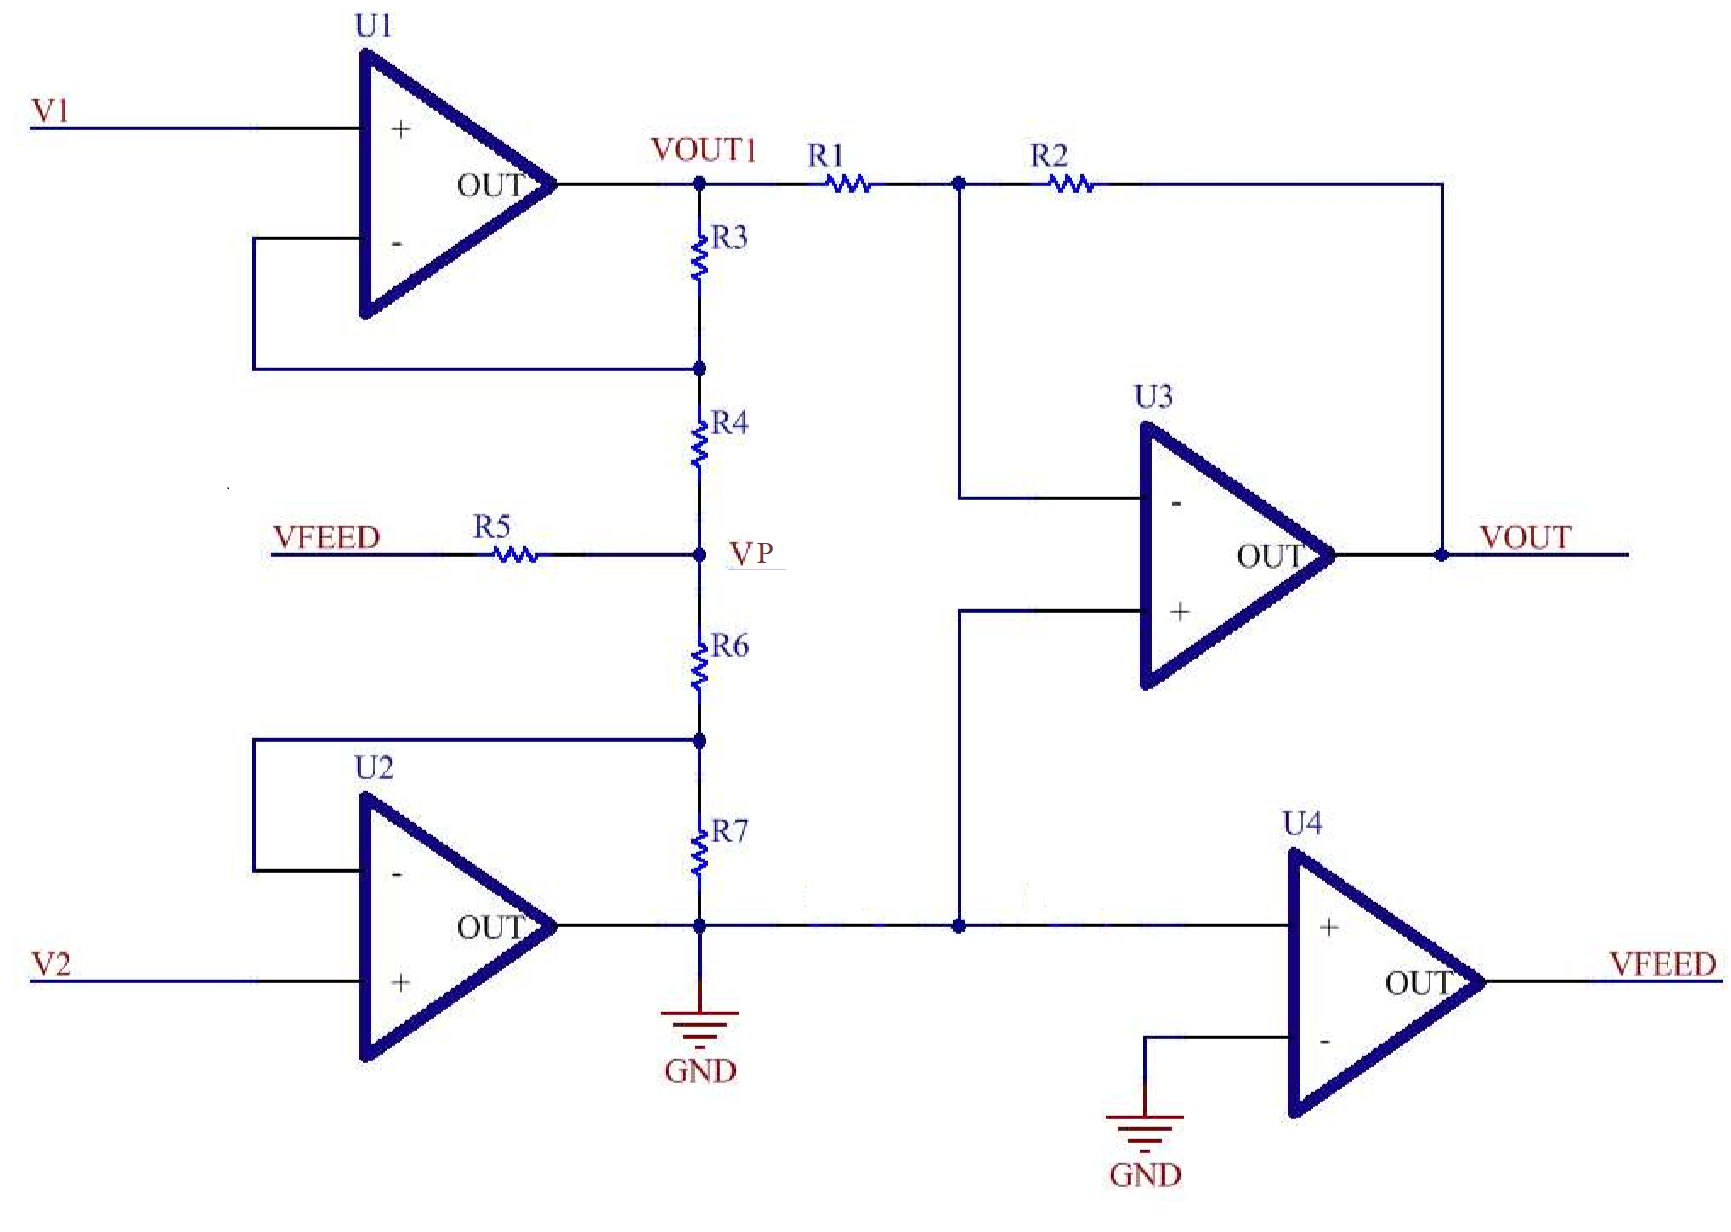
\includegraphics[scale=0.4]{imagenes/circuito_ideal.png}
		\caption{Circuito resultante con opamps ideales}
		\label{fig:ej3_circuito_ideal}
	\end{figure}
Por lo que, usando divisor resistivo, se plantea el siguiente sistema de ecuaciones: \par

%sistema de ecuaciones con opamp ideales
 	\begin{equation}
  	   \left\{
	  	    \begin{array}{ll}
		 					\mathrm{\frac{V_p}{R_4} - V_1\cdot (\frac{1}{R_4} + \frac{1}{R_3}) + \frac{V_{out1}}{R_3} = 0 } \\
			 				\mathrm{\frac{V_p}{R_6} - V_2\cdot (\frac{1}{R_6} + \frac{1}{R_7}) = 0 } \\
			 				\mathrm{\frac{V_{out1}}{R_1} + \frac{V_{out}}{R_2} = 0 } \\
	     	 \end{array}
	     	\right.
 	\end{equation}
 	
del cual se puede calcular la señal de salida en función de las entradas como: \par

$V_{out} = \frac{R_2\cdot [R_3\cdot (R_6 + R_7) \cdot V_2 -R_7\cdot (R_4 + R_3)\cdot V_1]}{R_1\cdot R_4\cdot R_7}$

Dado que se requiere que la salida sea directamente proporcional a la resta de las dos señales, para eliminar el modo común, se pide que:\par
\begin{centering}
$R_3\cdot (R_6 + R_7) = R_7\cdot (R_4 + R_3)$\par
\end{centering}
que resulta en la condición: \par
\begin{centering}
$\frac{R_3}{R_4} = \frac{R_7}{R_6}$\par
\end{centering}
Y cuya función transferencia final es: \par
$V_{out} = \frac{R_2\cdot R_7\cdot (R_4 + R_3)}{R_1\cdot R_4 \cdot R_7}\cdot (V_1 - V_2)$\par
Entonces: \par

%funcion transferencia ideal
\fbox{
				\centering
       $V_{out} = \frac{R_2}{R_1}\cdot (1 + \frac{R_3}{R_4})\cdot (V_1 - V_2)$
}

Esta relación ideal muestra una ganancia potencialmente grande y, tomando a la resta de la señales de entrada como la entrada de la transferencia, constante para todas las frecuencias. De esta manera el modelo ideal cumple efectivamente con el modelo de un amplificador de instrumentación.\par

Luego, en el contexto ideal, si se requiere una ganancia $X$, se puede solucionar este problema mediante las siguientes asignaciones: \par
 	\begin{equation}
  	   \left\{
	  	    \begin{array}{ll}
		 					\mathrm{\sqrt{X} = \frac{R_2}{R_1} } \\
			 				\mathrm{\sqrt{X} - 1 = \frac{R_3}{R_4}} \\
	     	 \end{array}
	     	\right.
 	\end{equation}
 	por lo que la razón $\frac{R_7}{R_6}$ quedaría también determinada como $\frac{R_7}{R_6} = \sqrt{X} - 1$ por la relación antes propuesta.

\subsection{Análisis \underline{NO} ideal del circuito}
\section{Simulaciones}

\section{Mediciones}

\section{Conclusión}

\end{document}
